\documentclass[final,serif,hyperref={pdfpagelabels=false}]{beamer}

\mode<presentation>
{
  \usetheme{nps}
}
\usepackage{grffile}
%\mode<presentation>{\usetheme{default}}
\usepackage[english]{babel}
\usepackage[latin1]{inputenc}
\usepackage{amsmath,amsthm, amssymb, latexsym}
%\usepackage[orientation=portrait,size=a0,scale=1.4,debug]{beamerposter}
\usepackage[orientation=landscape,size=custom,width=16,height=9,scale=0.5,debug]{beamerposter}
\usepackage[absolute,showboxes,overlay]{textpos}


\usepackage{tikz}
\usepackage{tikzpagenodes}
\usetikzlibrary{positioning,backgrounds}
\usetikzlibrary{shadows.blur}
\usetikzlibrary{shapes.symbols}
\usefonttheme{serif}

%\beamertemplatenavigationsymbolsempty

% light-colored theme
% title background color RGB: 228, 224, 221
% slide top-bar color RGB: 135, 126, 109
\definecolor{titlebg}{RGB}{228,224,221}
\definecolor{topbar}{RGB}{135,126,109}
% dark-colored theme


\setlength{\TPHorizModule}{10em}
\setlength{\TPVertModule}{\TPHorizModule}

\defbeamertemplate*{title page}{customized}[1][]
{
\vspace{8em}\centering
  \usebeamerfont{title}\inserttitle\par
  \usebeamerfont{subtitle} %\usebeamercolor[fg]{subtitle}
  \insertsubtitle\par
  \bigskip
  \usebeamerfont{author}\insertauthor\par
  \usebeamerfont{institute}\insertinstitute\par
  \usebeamerfont{date}\insertdate\par
  \usebeamercolor[fg]{titlegraphic}\inserttitlegraphic
}

%\setbeamertemplate{footline}[frame number]
\setbeamertemplate{sidebar right}{}
\setbeamertemplate{footline}{%
\hfill\usebeamertemplate***{navigation symbols}
\hspace{0.25cm}\insertframenumber{}/\inserttotalframenumber
}

\setbeamertemplate{frametitle}{
\hspace{-0.4cm}
%\vskip-0.01cm
  \strut\insertframetitle\strut
%\vspace{0.1cm}
%\vbox{\hsize=10cm\bfseries\strut\insertframetitle\strut}
%\vspace{0.1cm}
}



\title[Short Title]{NPS Themed Beamer Template}
\subtitle[Short subtitle]{A subtitle}
\author[T. Axtell]{Travis W. Axtell}
\institute[NPS]{Department of Electrical and Computer Engineering\\
Monterey, CA 93943}
\date[\today]{\today}

\begin{document}

% This creates the cover slide using the above information (do not change)
{
%\makeatletter % to change template
%    \setbeamertemplate{headline}[default] % not mandatory, but I though it 
%%was 
%    %better to set it blank
%    \def\beamer@entrycode{\vspace*{-\headheight}} % here is the part we are 
%    %interested in :)
%\makeatother
\setbeamertemplate{headline}
{\vspace*{-\headheight}
}
\usebackgroundtemplate{
%\setlength{\unitlength}{1em}
%\begin{picture}(1em,2em)
%\put(10em,10em){ 
\includegraphics[width=4em]{npsglobe}
%}
%\end{picture}
\hspace{-1em}
\begin{picture}(250,250)
\put(0,0){
\begin{tikzpicture}
\node (img1)  at (0,0) 
{
\includegraphics[width=1.25\textwidth]{backgroundlight}};
\end{tikzpicture}
}
\put(280,0){
\begin{tikzpicture}
\node (img1)  at (0,0) 
{
\includegraphics[width=15em]{npsglobe}};
\end{tikzpicture}
}
\put(200,150){
\begin{tikzpicture}
\node (img1)  at (0,0) 
{
\includegraphics[scale=0.25]{npslogovert}};
\end{tikzpicture}
}
\put(0,0){
\begin{tikzpicture}
\node (img1)  at (0,0) 
{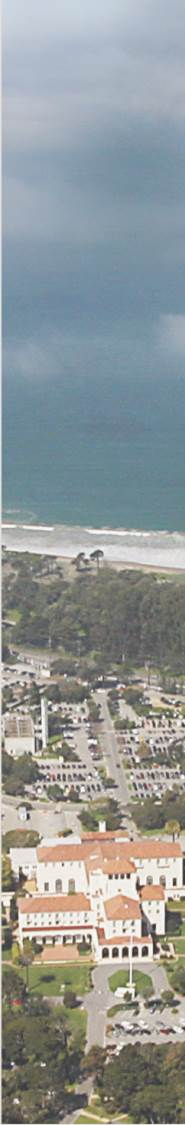
\includegraphics[height=\textheight]{sidepicture}};
\end{tikzpicture}
}
\end{picture}
}
\begin{frame}
\titlepage
\end{frame}
}

% This sets the background slide style for slide2 and beyond (do not change)
\makeatletter

\mode<presentation>

\usesectionheadtemplate
  {\hfill\insertsectionhead}
  {\hfill\color{fg!50!bg}\insertsectionhead}

\setbeamertemplate{headline}
{%
  \leavevmode%
  \@tempdimb=2.4375ex%
  \ifnum\beamer@subsectionmax<\beamer@sectionmax%
    \multiply\@tempdimb by\beamer@sectionmax%
  \else%
    \multiply\@tempdimb by\beamer@subsectionmax%
  \fi%
  \ifdim\@tempdimb>0pt%
    \advance\@tempdimb by 1.825ex%
    \begin{beamercolorbox}[wd=.5\paperwidth,ht=\@tempdimb]{section in 
    head/foot}%
      \vbox 
      to\@tempdimb{\vfil\insertsectionnavigation{.5\paperwidth}\vfil}%
    \end{beamercolorbox}%
    \begin{beamercolorbox}[wd=.5\paperwidth,ht=\@tempdimb]{subsection in 
    head/foot}%
      \vbox 
to\@tempdimb{\vfil\insertsubsectionnavigation{.5\paperwidth}\vfil}%
    \end{beamercolorbox}
  \fi
  %\vspace*{-\headheight}
}

\usebackgroundtemplate{
\hspace{-1em}
\begin{picture}(250,250)
\put(0,0){
\begin{tikzpicture}
\node (img1)  at (0,0) 
{
\includegraphics[width=1.25\textwidth]{backgroundlight}};
\end{tikzpicture}
}
\put(280,0){
\begin{tikzpicture}
\node (img1)  at (0,0) 
{
\includegraphics[width=15em]{npsglobe}};
\end{tikzpicture}
}
\put(0,0){
\begin{tikzpicture}
\node (img1)  at (0,0) 
{
\includegraphics[height=\textheight]{sidepicturethin}};
\end{tikzpicture}
}
\put(0,215) %x=25 for no overlap with sidepicturethin
{
\begin{tikzpicture}[opacity=0.6]
\fill [topbar,blur shadow={shadow blur steps=5}] (30,10) rectangle (5,5);
\end{tikzpicture}
}
\end{picture}
}

\setbeamertemplate{frametitle}{
%\hspace{-0.4cm}
\vskip1em
  \strut\insertframetitle\strut
%\vspace{0.1cm}
%\vbox{\hsize=10cm\bfseries\strut\insertframetitle\strut}
%\vspace{0.1cm}
}

\makeatother

% Your slide content follows (change these)

% Slides can be grouped into sections
\section{important section 1}

{


\subsection{Timely subsection}

% All slide content is in the frame environment.
\begin{frame}{A sample slide 1}

A displayed formula:

\[
  \int_{-\infty}^\infty e^{-x^2} \, dx = \sqrt{\pi}
\]

An itemized list:

\begin{itemize}
  \item itemized item 1
  \item itemized item 2
  \item itemized item 3
\end{itemize}

\begin{block}{Test block headline}
  In a right triangle, the square of hypotenuse equals
  the sum of squares of two other sides.
\end{block}

\end{frame}


\begin{frame}{A sample slide 2}

A displayed formula:

\[
  \int_{-\infty}^\infty e^{-x^2} \, dx = \sqrt{\pi}
\]

An itemized list:

\begin{itemize}
  \item itemized item 1
  \item itemized item 2
  \item itemized item 3
\end{itemize}

\begin{beamerboxesrounded}[upper=uppercol,lower=lowercol,shadow=true]{Theorem}
$A = B$.
\end{beamerboxesrounded}

\end{frame}

\begin{frame}{A sample slide 3}

A displayed formula:

\[
  \int_{-\infty}^\infty e^{-x^2} \, dx = \sqrt{\pi}
\]

An itemized list:

\begin{itemize}
  \item itemized item 1
  \item itemized item 2
  \item itemized item 3
\end{itemize}

\setbeamercolor{uppercol}{fg=white,bg=structure}%
\setbeamercolor{lowercol}{fg=black,bg=white}%
\begin{beamerboxesrounded}[upper=uppercol,lower=lowercol,shadow=true]
{Fundamental Theorem of Dullness}
$A = B$,\\
$C = D$.
\end{beamerboxesrounded}

\end{frame}

\section{very important section 2}

\begin{frame}{A sample slide 4}

A displayed formula:

\[
  \int_{-\infty}^\infty e^{-x^2} \, dx = \sqrt{\pi}
\]

An itemized list:

\begin{itemize}
  \item itemized item 1
  \item itemized item 2
  \item itemized item 3
\end{itemize}

\begin{theorem}
  In a right triangle, the square of hypotenuse equals
  the sum of squares of two other sides.
\end{theorem}

\end{frame}

\subsection{Subsection 2}

\begin{frame}{A sample slide 5}

A displayed formula:

\[
  \int_{-\infty}^\infty e^{-x^2} \, dx = \sqrt{\pi}
\]

An itemized list:

\begin{itemize}
  \item itemized item 1
  \item itemized item 2
  \item itemized item 3
\end{itemize}

\begin{theorem}
  In a right triangle, the square of hypotenuse equals
  the sum of squares of two other sides.
\end{theorem}

\end{frame}

\begin{frame}{A sample slide 6}

A displayed formula:

\[
  \int_{-\infty}^\infty e^{-x^2} \, dx = \sqrt{\pi}
\]

An itemized list:

\begin{itemize}
  \item itemized item 1
  \item itemized item 2
  \item itemized item 3
\end{itemize}

\begin{theorem}
  In a right triangle, the square of hypotenuse equals
  the sum of squares of two other sides.
\end{theorem}

\end{frame}

}

\end{document}
